%% bare_conf.tex
%% V1.4
%% 2012/12/27
%% by Michael Shell
%% See:
%% http://www.michaelshell.org/
%% for current contact information.
%%
%% This is a skeleton file demonstrating the use of IEEEtran.cls
%% (requires IEEEtran.cls version 1.8 or later) with an IEEE conference paper.
%%
%% Support sites:
%% http://www.michaelshell.org/tex/ieeetran/
%% http://www.ctan.org/tex-archive/macros/latex/contrib/IEEEtran/
%% and
%% http://www.ieee.org/

%%*************************************************************************
%% Legal Notice:
%% This code is offered as-is without any warranty either expressed or
%% implied; without even the implied warranty of MERCHANTABILITY or
%% FITNESS FOR A PARTICULAR PURPOSE! 
%% User assumes all risk.
%% In no event shall IEEE or any contributor to this code be liable for
%% any damages or losses, including, but not limited to, incidental,
%% consequential, or any other damages, resulting from the use or misuse
%% of any information contained here.
%%
%% All comments are the opinions of their respective authors and are not
%% necessarily endorsed by the IEEE.
%%
%% This work is distributed under the LaTeX Project Public License (LPPL)
%% ( http://www.latex-project.org/ ) version 1.3, and may be freely used,
%% distributed and modified. A copy of the LPPL, version 1.3, is included
%% in the base LaTeX documentation of all distributions of LaTeX released
%% 2003/12/01 or later.
%% Retain all contribution notices and credits.
%% ** Modified files should be clearly indicated as such, including  **
%% ** renaming them and changing author support contact information. **
%%
%% File list of work: IEEEtran.cls, IEEEtran_HOWTO.pdf, bare_adv.tex,
%%                    bare_conf.tex, bare_jrnl.tex, bare_jrnl_compsoc.tex,
%%                    bare_jrnl_transmag.tex
%%*************************************************************************

% *** Authors should verify (and, if needed, correct) their LaTeX system  ***
% *** with the testflow diagnostic prior to trusting their LaTeX platform ***
% *** with production work. IEEE's font choices can trigger bugs that do  ***
% *** not appear when using other class files.                            ***
% The testflow support page is at:
% http://www.michaelshell.org/tex/testflow/



% Note that the a4paper option is mainly intended so that authors in
% countries using A4 can easily print to A4 and see how their papers will
% look in print - the typesetting of the document will not typically be
% affected with changes in paper size (but the bottom and side margins will).
% Use the testflow package mentioned above to verify correct handling of
% both paper sizes by the user's LaTeX system.
%
% Also note that the "draftcls" or "draftclsnofoot", not "draft", option
% should be used if it is desired that the figures are to be displayed in
% draft mode.
%
\documentclass[conference]{IEEEtran}
% Add the compsoc option for Computer Society conferences.
%
% If IEEEtran.cls has not been installed into the LaTeX system files,
% manually specify the path to it like:
% \documentclass[conference]{../sty/IEEEtran}



% Some very useful LaTeX packages include:
% (uncomment the ones you want to load)


% For directly writing german umlauts uncomment the appropriate line for
% your operating system:
% Windows:
% \usepackage[ansinew]{inputenc}
% Linux:
%\usepackage[latin1]{inputenc}
% Mac
% \usepackage[applemac]{inputenc}
% If none of the above lines work you can also try the following:
\usepackage[utf8]{inputenc}



% *** MISC UTILITY PACKAGES ***
%
%\usepackage{ifpdf}
% Heiko Oberdiek's ifpdf.sty is very useful if you need conditional
% compilation based on whether the output is pdf or dvi.
% usage:
% \ifpdf
%   % pdf code
% \else
%   % dvi code
% \fi
% The latest version of ifpdf.sty can be obtained from:
% http://www.ctan.org/tex-archive/macros/latex/contrib/oberdiek/
% Also, note that IEEEtran.cls V1.7 and later provides a builtin
% \ifCLASSINFOpdf conditional that works the same way.
% When switching from latex to pdflatex and vice-versa, the compiler may
% have to be run twice to clear warning/error messages.



% *** CITATION PACKAGES ***
%
\usepackage{cite}
% cite.sty was written by Donald Arseneau
% V1.6 and later of IEEEtran pre-defines the format of the cite.sty package
% \cite{} output to follow that of IEEE. Loading the cite package will
% result in citation numbers being automatically sorted and properly
% "compressed/ranged". e.g., [1], [9], [2], [7], [5], [6] without using
% cite.sty will become [1], [2], [5]--[7], [9] using cite.sty. cite.sty's
% \cite will automatically add leading space, if needed. Use cite.sty's
% noadjust option (cite.sty V3.8 and later) if you want to turn this off
% such as if a citation ever needs to be enclosed in parenthesis.
% cite.sty is already installed on most LaTeX systems. Be sure and use
% version 4.0 (2003-05-27) and later if using hyperref.sty. cite.sty does
% not currently provide for hyperlinked citations.
% The latest version can be obtained at:
% http://www.ctan.org/tex-archive/macros/latex/contrib/cite/
% The documentation is contained in the cite.sty file itself.






% *** GRAPHICS RELATED PACKAGES ***
%
\ifCLASSINFOpdf
  \usepackage[pdftex]{graphicx}
  % declare the path(s) where your graphic files are
  % \graphicspath{{../pdf/}{../jpeg/}}
  % and their extensions so you won't have to specify these with
  % every instance of \includegraphics
  % \DeclareGraphicsExtensions{.pdf,.jpeg,.png}
\else
  % or other class option (dvipsone, dvipdf, if not using dvips). graphicx
  % will default to the driver specified in the system graphics.cfg if no
  % driver is specified.
  \usepackage[dvips]{graphicx}
  % declare the path(s) where your graphic files are
  % \graphicspath{{../eps/}}
  % and their extensions so you won't have to specify these with
  % every instance of \includegraphics
  % \DeclareGraphicsExtensions{.eps}
\fi
% graphicx was written by David Carlisle and Sebastian Rahtz. It is
% required if you want graphics, photos, etc. graphicx.sty is already
% installed on most LaTeX systems. The latest version and documentation
% can be obtained at: 
% http://www.ctan.org/tex-archive/macros/latex/required/graphics/
% Another good source of documentation is "Using Imported Graphics in
% LaTeX2e" by Keith Reckdahl which can be found at:
% http://www.ctan.org/tex-archive/info/epslatex/
%
% latex, and pdflatex in dvi mode, support graphics in encapsulated
% postscript (.eps) format. pdflatex in pdf mode supports graphics
% in .pdf, .jpeg, .png and .mps (metapost) formats. Users should ensure
% that all non-photo figures use a vector format (.eps, .pdf, .mps) and
% not a bitmapped formats (.jpeg, .png). IEEE frowns on bitmapped formats
% which can result in "jaggedy"/blurry rendering of lines and letters as
% well as large increases in file sizes.
%
% You can find documentation about the pdfTeX application at:
% http://www.tug.org/applications/pdftex





% *** MATH PACKAGES ***
\usepackage[cmex10]{amsmath}
% A popular package from the American Mathematical Society that provides
% many useful and powerful commands for dealing with mathematics. If using
% it, be sure to load this package with the cmex10 option to ensure that
% only type 1 fonts will utilized at all point sizes. Without this option,
% it is possible that some math symbols, particularly those within
% footnotes, will be rendered in bitmap form which will result in a
% document that can not be IEEE Xplore compliant!
%
% Also, note that the amsmath package sets \interdisplaylinepenalty to 10000
% thus preventing page breaks from occurring within multiline equations. Use:
\interdisplaylinepenalty=2500
% after loading amsmath to restore such page breaks as IEEEtran.cls normally
% does. amsmath.sty is already installed on most LaTeX systems. The latest
% version and documentation can be obtained at:
% http://www.ctan.org/tex-archive/macros/latex/required/amslatex/math/





% *** SPECIALIZED LIST PACKAGES ***
%
%\usepackage{algorithmic}
% algorithmic.sty was written by Peter Williams and Rogerio Brito.
% This package provides an algorithmic environment fo describing algorithms.
% You can use the algorithmic environment in-text or within a figure
% environment to provide for a floating algorithm. Do NOT use the algorithm
% floating environment provided by algorithm.sty (by the same authors) or
% algorithm2e.sty (by Christophe Fiorio) as IEEE does not use dedicated
% algorithm float types and packages that provide these will not provide
% correct IEEE style captions. The latest version and documentation of
% algorithmic.sty can be obtained at:
% http://www.ctan.org/tex-archive/macros/latex/contrib/algorithms/
% There is also a support site at:
% http://algorithms.berlios.de/index.html
% Also of interest may be the (relatively newer and more customizable)
% algorithmicx.sty package by Szasz Janos:
% http://www.ctan.org/tex-archive/macros/latex/contrib/algorithmicx/




% *** ALIGNMENT PACKAGES ***
%
%\usepackage{array}
% Frank Mittelbach's and David Carlisle's array.sty patches and improves
% the standard LaTeX2e array and tabular environments to provide better
% appearance and additional user controls. As the default LaTeX2e table
% generation code is lacking to the point of almost being broken with
% respect to the quality of the end results, all users are strongly
% advised to use an enhanced (at the very least that provided by array.sty)
% set of table tools. array.sty is already installed on most systems. The
% latest version and documentation can be obtained at:
% http://www.ctan.org/tex-archive/macros/latex/required/tools/


% IEEEtran contains the IEEEeqnarray family of commands that can be used to
% generate multiline equations as well as matrices, tables, etc., of high
% quality.
\usepackage{threeparttable}



% *** SUBFIGURE PACKAGES ***
\ifCLASSOPTIONcompsoc
 \usepackage[caption=false,font=normalsize,labelfont=sf,textfont=sf]{subfig}
\else
 \usepackage[caption=false,font=footnotesize]{subfig}
\fi
% subfig.sty, written by Steven Douglas Cochran, is the modern replacement
% for subfigure.sty, the latter of which is no longer maintained and is
% incompatible with some LaTeX packages including fixltx2e. However,
% subfig.sty requires and automatically loads Axel Sommerfeldt's caption.sty
% which will override IEEEtran.cls' handling of captions and this will result
% in non-IEEE style figure/table captions. To prevent this problem, be sure
% and invoke subfig.sty's "caption=false" package option (available since
% subfig.sty version 1.3, 2005/06/28) as this is will preserve IEEEtran.cls
% handling of captions.
% Note that the Computer Society format requires a larger sans serif font
% than the serif footnote size font used in traditional IEEE formatting
% and thus the need to invoke different subfig.sty package options depending
% on whether compsoc mode has been enabled.
%
% The latest version and documentation of subfig.sty can be obtained at:
% http://www.ctan.org/tex-archive/macros/latex/contrib/subfig/




% *** FLOAT PACKAGES ***
%
%\usepackage{fixltx2e}
% fixltx2e, the successor to the earlier fix2col.sty, was written by
% Frank Mittelbach and David Carlisle. This package corrects a few problems
% in the LaTeX2e kernel, the most notable of which is that in current
% LaTeX2e releases, the ordering of single and double column floats is not
% guaranteed to be preserved. Thus, an unpatched LaTeX2e can allow a
% single column figure to be placed prior to an earlier double column
% figure. The latest version and documentation can be found at:
% http://www.ctan.org/tex-archive/macros/latex/base/


%\usepackage{stfloats}
% stfloats.sty was written by Sigitas Tolusis. This package gives LaTeX2e
% the ability to do double column floats at the bottom of the page as well
% as the top. (e.g., "\begin{figure*}[!b]" is not normally possible in
% LaTeX2e). It also provides a command:
%\fnbelowfloat
% to enable the placement of footnotes below bottom floats (the standard
% LaTeX2e kernel puts them above bottom floats). This is an invasive package
% which rewrites many portions of the LaTeX2e float routines. It may not work
% with other packages that modify the LaTeX2e float routines. The latest
% version and documentation can be obtained at:
% http://www.ctan.org/tex-archive/macros/latex/contrib/sttools/
% Do not use the stfloats baselinefloat ability as IEEE does not allow
% \baselineskip to stretch. Authors submitting work to the IEEE should note
% that IEEE rarely uses double column equations and that authors should try
% to avoid such use. Do not be tempted to use the cuted.sty or midfloat.sty
% packages (also by Sigitas Tolusis) as IEEE does not format its papers in
% such ways.
% Do not attempt to use stfloats with fixltx2e as they are incompatible.
% Instead, use Morten Hogholm'a dblfloatfix which combines the features
% of both fixltx2e and stfloats:
%
% \usepackage{dblfloatfix}
% The latest version can be found at:
% http://www.ctan.org/tex-archive/macros/latex/contrib/dblfloatfix/




% *** PDF, URL AND HYPERLINK PACKAGES ***
%
%\usepackage{url}
% url.sty was written by Donald Arseneau. It provides better support for
% handling and breaking URLs. url.sty is already installed on most LaTeX
% systems. The latest version and documentation can be obtained at:
% http://www.ctan.org/tex-archive/macros/latex/contrib/url/
% Basically, \url{my_url_here}.




% *** Do not adjust lengths that control margins, column widths, etc. ***
% *** Do not use packages that alter fonts (such as pslatex).         ***
% There should be no need to do such things with IEEEtran.cls V1.6 and later.
% (Unless specifically asked to do so by the journal or conference you plan
% to submit to, of course. )

% add custom packages
\usepackage{color}
\definecolor{tumblue}{rgb}{0, 0.4, 0.74}



% correct bad hyphenation here
\hyphenation{op-tical net-works semi-conduc-tor}


\begin{document}

% Add the seminar's cover page
\begin{figure*}[!ht]
  
\includegraphics{./images/IN.pdf} \hfill 
\includegraphics{./images/tumlogo.pdf}
 
  \vspace*{1cm}
  {\large \textsf{Fakult{\"a}t f{\"u}r Informatik}}\\
  {\large \textsf{Lehrstuhl f{\"u}r Echtzeitsysteme und Robotik}}\\
   

  \vspace*{5cm}
%
%
% TITEL DER ARBEIT
%
%
  {\color{tumblue} \Huge \bf \textsf{Numerical Inverse Kinematics in Cluttered Environments}}\\

  \vspace*{1cm}
%
%
% NAME DES STUDENTEN (auf Titelblatt)
%
% 
  {\Large \bf \textsf{Emanuel André Medina Araujo}}\\   % HIER EINSETZEN!
 
  \vspace*{8cm}
  {\Large \textsf{Seminar \emph{Cyber-Physical Systems} ST 2023}}\\
 
  \vspace*{1cm} 
  \begin{tabular}{ll}
%
%
% NAME DES BETREUERS
%
%
    {\Large \bf \textsf{Advisor:}} &
    {\Large \textsf{Jonathan Külz}}\\                  % HIER EINSETZEN!
    \\

    {\Large \bf \textsf{Supervisor:}} &
    {\Large \textsf{Prof.~Dr.-Ing. Matthias Althoff}}\\
    \\

%
%
% ABGABETERMIN
%
%
    {\Large \bf \textsf{Submission:}} &
    {\Large \textsf{31. July 2023}}

  \end{tabular}
  
\end{figure*}


%
% paper title
% can use linebreaks \\ within to get better formatting as desired
% Do not put math or special symbols in the title.
\title{Numerical Inverse Kinematics in Cluttered Environments}


% author names and affiliations
% use a multiple column layout for up to three different
% affiliations
\author{\IEEEauthorblockN{Emanuel André Medina Araujo}
\IEEEauthorblockA{Technische Universit\"at M\"unchen\\
Email: emanuel.medina@tum.de}}

% conference papers do not typically use \thanks and this command
% is locked out in conference mode. If really needed, such as for
% the acknowledgment of grants, issue a \IEEEoverridecommandlockouts
% after \documentclass

% use for special paper notices
%\IEEEspecialpapernotice{(Invited Paper)}



% make the title area
\maketitle

% As a general rule, do not put math, special symbols or citations
% in the abstract
\begin{abstract}
Nowadays, robots are often modeled and built redundantly with multiple degrees of freedom (DOF) needing to move around in complex environments. This report presents an overview of the most common numerical approaches to the Inverse Kinematics (IK) problem in cluttered environments. The mentioned use cases are active research topics based on the IK problem, making it indispensable.

Depending on the task, the IK problem can result as unsolvable, in a single solution, or a multitude of solutions, preventing a general analytical approach. Herefore many numerical methods have been proposed, which we will analyze and compare in this report. Due to the multimodality of the problem, we will further restrict ourselves to the class of Jacobian methods, heuristic methods, and meta-heuristic methods.
Each method class will be introduced and inspected for the secondary obstacle avoidance task.
Afterward, the presented methods will be compared to each other.

Results show that Heuristic and Meta-Heuristic Methods are the best options for solving the IK problem numerically in cluttered environments in a general way.
\end{abstract}
% no keywords


% For peer review papers, you can put extra information on the cover
% page as needed:
% \ifCLASSOPTIONpeerreview
% \begin{center} \bfseries EDICS Category: 3-BBND \end{center}
% \fi
%
% For peerreview papers, this IEEEtran command inserts a page break and
% creates the second title. It will be ignored for other modes.
\IEEEpeerreviewmaketitle



\section{Introduction}
% no \IEEEPARstart
In various widely spread fields, the Inverse Kinematics (IK) problem is predominant. Let it be the control of figures and simulations in the animation industry, an agriculture robot in charge of harvesting fruits without hitting any branches, an assisting surgical robot that is supposed to move to a target position without hurting the patient, or many more. For simplicity, we will restrict ourselves to the field of robotics. Nonetheless, the presented methods may also be compatible with different applications using a modified version.

Ever since the industry's increasing robot automation\cite{Chiacchio2018impact}, the IK of numerous manipulators have to be calculated. Manipulators are often built with many degrees of freedom (DOF) to solve various complex tasks. That ends in the IK of a kinematically-redundant manipulator 
varying from being unsolvable to having infinite solutions. Only some manipulators IK can be calculated analytically\cite{springer_Kinematics}. Although existing approaches exist to solve the IK analytically\cite{chen_analyticalSolver} \cite{manocha_analyticalSolver}, recent research trends have shown that numerical methods are not restricting with increasing DOF. Since analytical methods have to be calculated for each manipulator individually, high engineering fees arise each time a robot is adapted even slightly. In contrast, numerical methods have vast application possibilities since the modification needed for a manipulator is manageable and implemented way faster than solving the system analytically. Based on that, we will further restrict ourselves to numerical methods for solving the IK problem.

In general, we will be classifying the presented methods into three categories. First is the class of Jacobian methods \cite{springer_Kinematics}, which uses the Jacobian matrix to solve the IK of a given manipulator. The most popular approaches include the Jacobian Inverse, the Jacobian Transpose, and the (selectively) Damped Least Square method.
The second class of solutions is the class of heuristic methods. We will look into the cyclic coordinate descent method (CCD) first introduced in \cite{wang_combined_1991}, and the Forward And Backward Reaching Inverse Kinematics (FABRIK) method \cite{aristidou_fabrik_2011}. Third, the meta-heuristic methods will be presented. Here we will have a look at the Differential Evolutionary Algorithms(DEAs)\cite{zhang_research_2021} and the Particle Swarm Optimization (PSO) method \cite{yiyang_general_2021}.
One has to note that alternative methods exist that will not be discussed, for example, the Newton Methods \cite{fletcher_practical_2000}, the Monte Carlo Methods \cite{kwan_wu_chin_closed-form_1997}, Style or Mesh-based IK \cite{grochow_style-based_2004} \cite{sumner_mesh-based_2005}, the Sequential Inverse Kinematics method \cite{unzueta_full-body_2008} \cite{perales_predicting_2008}, and Feedback IK \cite{pechev_inverse_2008}.

Furthermore, the previously mentioned kinematically-redundant manipulators must cope with more challenges when used in the real world\cite{springer_motionPlanning_ObstacleAvoidance}. That includes (but not exclusively) the optimization of calculation time, minimization of energy consumption \cite{faraji_singularity-tolerant_2017}, joint limit avoidance \cite{goos_real-time_1998}, and many more \cite{kilin_experimental_2017} \cite{siciliano_kinematic_1990}. One is obstacle avoidance in cluttered environments, which has been researched actively \cite{maciejewski_obstacle_1985}. Two prominent examples are agriculture robots \cite{maciejewski_obstacle_1985} and surgical robots \cite{colan_concurrent_2023}.

The former is a result of the increasing demand for field cultivation. Especially seasonal crops are still in need of manual harvest. Despite recent advances in automation technology, the regional and seasonal workforce is coping with challenges like increasing salaries and hard working conditions for humans. Opposed to that, robots can harvest fruits individually, possibly around the clock without payment\cite{silwal_design_2017} \cite{pedersen_agricultural_2006} and without physically injuring anyone. In addition, the manipulator must reach the target while avoiding collisions with branches, trunks, or other obstacles. All in one, the literature discloses that robots have been used widely for harvesting applications \cite{belforte_robot_2006} \cite{hayashi_evaluation_2010} \cite{agricultural_2023}.

Surgical Robots would enable highly specialized doctors to operate on patients in remote places \cite{guthart_intuitivesup_2000} in preoperative planning \cite{hayashibe_preoperative_2005}. The IK problem with obstacle avoidance can be found when minimizing contact with the patient's body \cite{berthet-rayne_inverse_2018}. Moreover, during surgery, it can warn the surgeon of any human error and improve the surgery results \cite{kavoussi_comparison_1995}.

This report is structured as follows. Section 2 explains the inverse kinematics problem and obstacle avoidance strategies. Section 3 introduces and analyzes numerical methods for solving the inverse kinematics problem and discusses how obstacle avoidance can be combined. Here the presented methods will be compared in terms of usability for different use cases. Section 5 concludes and notes further real-world restrictions to consider.





\section{The Inverse Kinematics Problem and Obstacle Avoidance}
\subsection{The Inverse Kinematics problem}
The Inverse Kinematics (IK) problem is an essential aspect of robotics, aiming to receive a robot's or animated figure joint configurations corresponding to a desired target position. Unlike the forward kinematics problem, which involves calculating the position and orientation of the end-effector given the joint angles, the IK problem poses a more challenging task of finding the joint angles that produce a desired end-effector pose. Because a manipulator can possibly reach a certain position with various joint angles, the IK problem can vary from infinite solutions to unsolvable.

Solving the IK problem analytically can be complex and computationally expensive, especially for complex robotic systems with many DOF \cite{shimizu_analytical_2008}. Even though solving the IK problem analytically is highly accurate, some manipulators might lack an analytical solution, especially redundant manipulators \cite{conkur_buckingham_1997}. As a result, numerical approaches have gained significant attention due to their ability to handle complex kinematic structures and provide efficient solutions. Although some research exists for analytical solvers \cite{chen_analyticalSolver} \cite{manocha_analyticalSolver}, we will focus on current trends of the numerical approaches for solving the IK problem. 

Numerical methods for solving the IK problem involve iterative algorithms that gradually refine a starting estimate of the joint configurations until the desired end-effector position is achieved. These approaches rely on numerical optimization techniques, which aim to minimize an objective function that quantifies the discrepancy between the expected and achieved poses. On top, further constraints are often applied to these functions to fulfill specific requirements, one of which is obstacle avoidance in a cluttered environment.

\subsection{Obstacle avoidance}
In many use cases, manipulators have to operate in cluttered environments. Therefore a safe and efficient operation has to be ensured, by further constraining the IK problem.
\subsubsection{Primary and Secondary Tasks}
To achieve obstacle avoidance, it is essential to consider the concept of primary and secondary tasks. Primary tasks refer to the primary objectives of the robotic system, such as reaching a desired end-effector pose. In contrast, secondary tasks encompass additional purposes, such as avoiding collisions with environmental obstacles or constraints from the robot's mechanical structure, e.g., joint limits.

While the user often specifies the primary task, secondary tasks usually constrain the execution to comply with further restrictions. The challenge lies in finding an efficient solution for the primary tasks that complies best with the secondary task. That also includes collision-free movement.
\subsubsection{What is Obstacle Avoidance}
Obstacle Avoidance ensures that the robotic system's movements to their end-effector pose are collision-free while conserving the constraints of the robot's mechanical structure. Although the IK problem usually deals with the end-effector position, collisions can occur on every robot link.
The most common approach is utilizing the tight-fitting oriented bounding box method. In the following subsection, we will discuss this method in more detail.

\begin{figure}[!t]
\centering
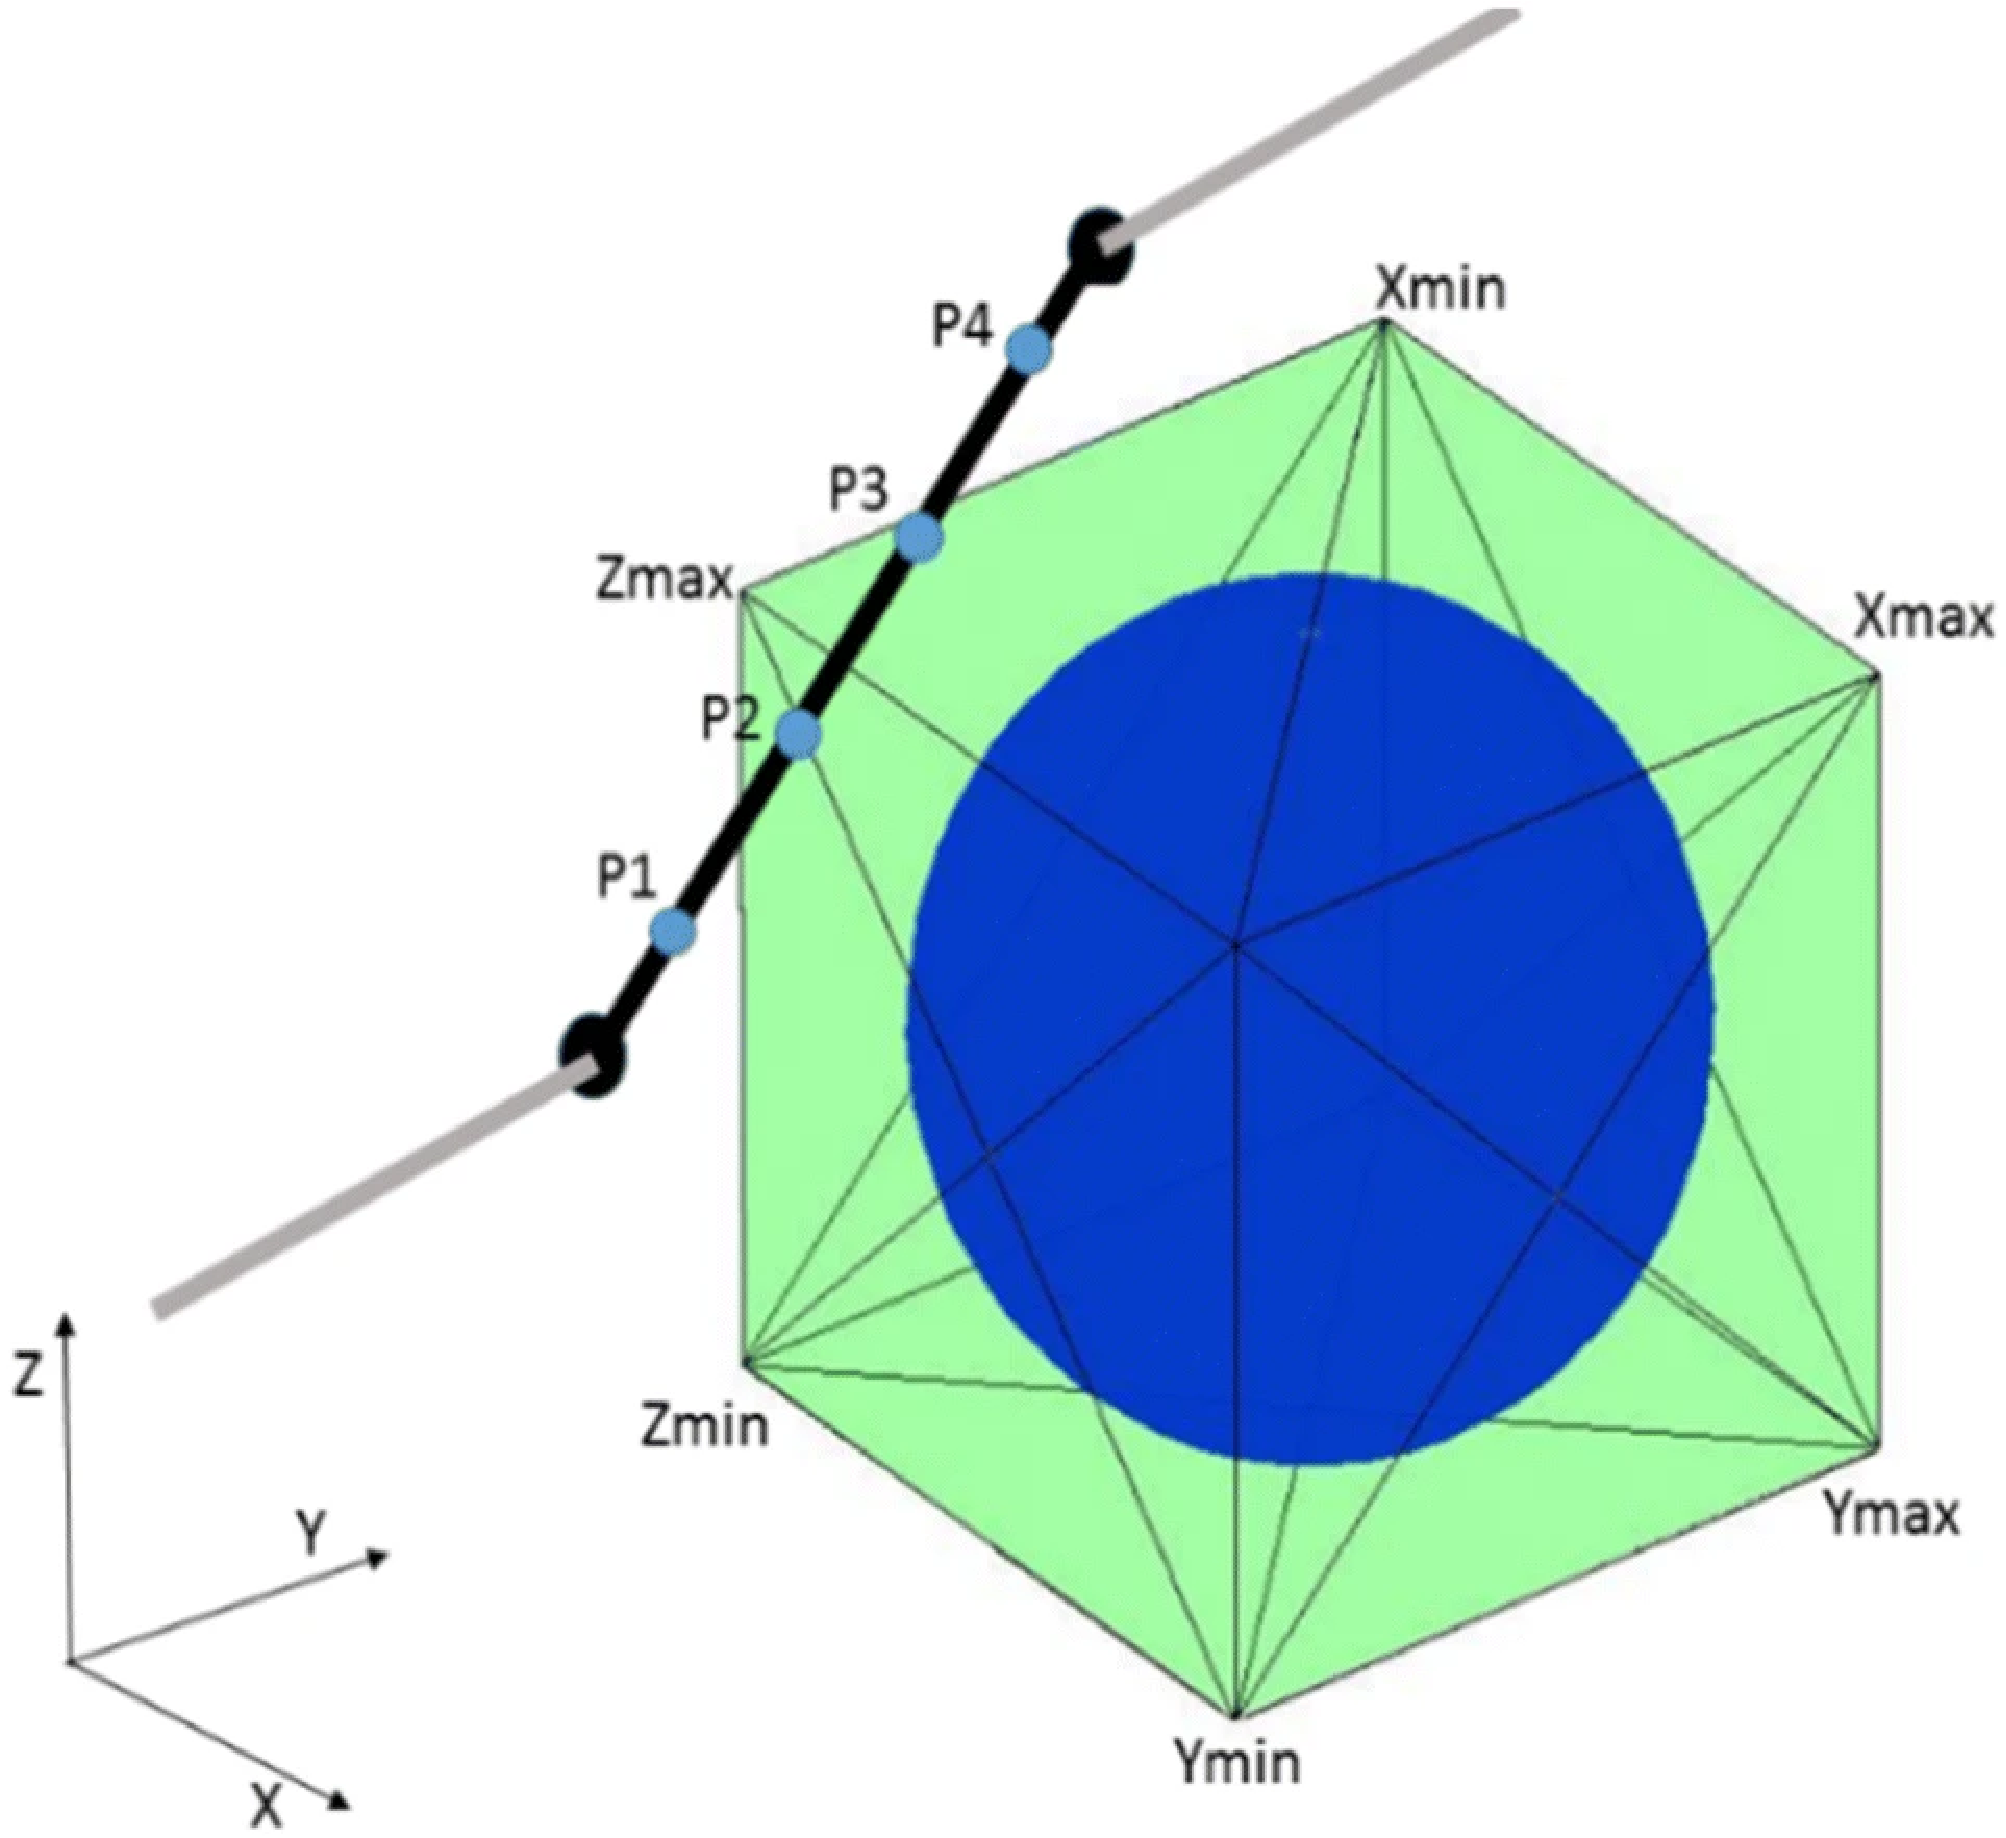
\includegraphics[width=2.5in]{images/TFOBB.pdf}
\caption{from\cite{chembuly_efficient_2020}. TFOBB of a spherical obstacle next to a manipulator link.}
\label{fig:TFOBB_Picture}
\end{figure}

\subsubsection{Tight-fitting Oriented Bounding Box}
The tight-fitting oriented bounding box (TFOBB) method is often used for obstacle avoidance in IK \cite{chembuly_efficient_2020} for simplifying calculations. It involves constructing bounding boxes around the robot's links and the surrounding obstacles (Fig. \ref{fig:TFOBB_Picture}). By comparing the bounding boxes, potential collisions can be detected. This can be helpful when we need to perform operations that may be inefficient to execute on the actual geometries due to the number of vertices. Especially when avoiding collision with humans, real-time calculations are needed in which the real geometries would be too time-consuming.
The TFOBB method aims to find joint angles that maximize the distance between the robot's links and the obstacles, ensuring that the IK solving is collision-free.
Moreover, the TFOBB method offers fast computation and is particularly suitable for environments with well-defined geometric obstacles. 

However, it may be less effective in environments with irregular or complex shapes, where the tight-fitting bounding boxes may need to accurately represent the collision regions. Research shows that optimizations have attempted to solve that problem by using various geometric forms \cite{barequet_efficiently_2001} \cite{held_evaluation_1995}.

TFOBB being a secondary task, we still need to explain methods for solving the IK problem as a primary task. This will be done in the following section.




\section{Numerical Methods for Solving the Inverse Kinematics Problem}\label{Numerical methods intro}
The last section introduced the TFOBB method for obstacle avoidance that can be put on top of the existing method to solve the IK problem. Many methods have been developed to refine the joint configurations to reach the end-effector pose. Based on a m-dimensional task space and n joint angles, we will define in a vector $\theta \in R^n$ for a manipulator with n DOF.
The following will introduce an overview of the most common numerical approaches for solving the IK problem and how the secondary task of obstacle avoidance can be achieved using them. These include the Jacobian Methods, Heuristic Methods, and Meta-Heuristic Methods. We will not discuss other methods classes in this report. Exemplarily, not discussed methods are the Newton Methods \cite{fletcher_practical_2000} \cite{kwan_wu_chin_closed-form_1997} which is an optimization approach, the Monte Carlo Method\cite{kwan_wu_chin_closed-form_1997}, the Sequential Monte Carlo Method \cite{perales_inverse_2008}, Neural Networks \cite{mao_obstacle_1997}, the Style or Mesh-based Method \cite{grochow_style-based_2004} \cite{sumner_mesh-based_2005}, the sequential Inverse Kinematics method \cite{perales_predicting_2008}, and Feedback IK \cite{pechev_inverse_2008}.

\subsection{Jacobian Methods}\label{JacobianMethods}
The Jacobian methods are the most commonly used class of solving techniques used for the inverse kinematics problem. These methods involve calculating the Jacobian matrix, representing the relationship between the joint and end-effector velocities. The relation between the end-effector's velocity $\dot{\vec{s}}$ and the joint velocity $\dot{\theta}$ can be given by:
\begin{equation}\label{eq:forwardKinematic}
    \dot{\vec{s}} = J\dot{\theta}
\end{equation}
where $J \in R^{m \times n}$ is the Jacobian matrix which can be seen as a function $J(\theta)$ of the angles $\theta$. We search the change in joint angles $\Delta\theta$ that can be estimated by $\Delta s \approx J\Delta\theta$ when choosing $\Delta \theta$ in a way so that $\Delta s$ is approximately equal to $\vec{e}$ by linearization.
Then IK problem can be solved when the Jacobian matrix is symmetric by reconfiguring the equation \eqref{eq:forwardKinematic} to:
\begin{equation}\label{eq:inverseKinematic}
    \Delta\theta = J^{-1}\vec{e}
\end{equation}
Otherwise, we can take advantage of the kinematically-redundant end-effectors by applying the following numerical Jacobian methods, each with strengths and limitations.

\subsubsection{Jacobian Transpose}
The Jacobian transpose method involves calculating the transpose of the Jacobian matrix and using it to find a solution for the change in joint angles. It was introduced by \cite{wolovich_computational_1984} \cite{balestrino_robust_1984} and calculates the change in joint angles using the following equation:
\begin{equation}
\Delta\theta = \alpha J^T\vec{e}
\end{equation}
where $\alpha$ is a positive scalar, and base idea is to replace the inverse with the transpose of the Jacobian matrix. If $\alpha$ is small enough, \cite{balestrino_robust_1984} and \cite{wolovich_computational_1984} showed that the error of approximating the inverse with the transpose is neglectable by justifying the use in terms of virtual forces. According to \cite{buss_introduction_2004}, it has a lower computational burden than fellow Jacobian methods since no inverses need to be calculated. However, it may not always provide an optimal solution, especially when multiple end-effectors come into play.

\subsubsection{Jacobian Pseudo Inverse}
The Jacobian pseudo-inverse method, also known as the Moore-Penrose inverse, calculates a pseudo-inverse of the Jacobian matrix $J$ because $J$ is most likely redundant \cite{springer_redundant} and non-square. Thus, an ordinary inverse is impossible. The pseudo-inverse of the Jacobian matrix $J^+$ can be calculated as follows:
\begin{equation}
J^+ = J^T(JJ^T)^{-1}
\end{equation}
The change in joint angles can then be calculated using the following equation:
\begin{equation}
\Delta\theta = J^+\vec{e}
\end{equation}
However, this method is volatile near singularities, which occurs when the Jacobian matrix is about to lose full rank. That usually happens when the end-effector is almost entirely extended, resulting in large changes in joint angles. Nonetheless, the Jacobian pseudo inverse method won't move in an impossible direction precisely at singularities and is, therefore, well-behaved. 

Additionally, the matrix $(I - J^+J)$ projects onto the nullspace of $J$. Applied to robotics, the nullspace comprises all changes in joint angles that result in no changes at the end effector position or orientation. Using the following equation, \cite{liegois_automatic_1977} first used the property that $J(I - J^+J)\phi = 0$ to avoid joint limits:
\begin{equation}
\Delta\theta = J^+\vec{e} + (I - J^+J)\phi
\end{equation}
This is called the nullspace method, and $\phi$ can be used for secondary tasks and/or prioritizing various tasks \cite{baerlocher_task-priority_1998} \cite{chiaverini_singularity-robust_1997}. 

In practice, the pseudo inverse method is rarely used because of the near singularities' difficulties. Therefore, the Singular Value Decomposition and (selectively) Damped Least Squares methods are preferred due to their superior performance\cite{buss_selectively_2005}.

\subsubsection{Singular Value Decomposition}
Singular value decomposition (SVD) is a technique to decompose a matrix into constituent parts. In essence, the SVD assimilates the Pseudo Inverse Method rather than being a method in itself. It can be used to calculate the pseudo-inverse of the Jacobian matrix, which can then be used to solve the inverse kinematics problem. The SVD of the Jacobian matrix, J, can be calculated as follows:
\begin{equation}
J = U\Sigma V^T
\end{equation}
where U and V are orthogonal matrices, and $\Sigma$ is a diagonal matrix containing the singular values of J. The pseudo-inverse of J can then be calculated as follows:
\begin{equation}
J^+ = V\Sigma^+U^T
\end{equation}
where $\Sigma^+$ is the pseudo inverse of $\Sigma$. SVD is particularly useful when dealing with ill-conditioned or singular matrices because the singular value decomposition of the Jacobian always exists. This will be used to deduce the Selectively Damped Least Square method \cite{buss_selectively_2005}.

\subsubsection{Damped Least Squares}
The damped least squares (DLS) method involves adding a damping factor to the Jacobian matrix to improve the stability of the solution by preventing large joint velocities and avoiding many of the Pseudo Inverse method's problems. It was first introduced by \cite{wampler_manipulator_1986} and is based on the formula:
\begin{equation} \label{dampedLeastSquares}
\Delta\theta = J^T(JJ^T + \lambda^2I)^{-1}\vec{e}
\end{equation}
where $\lambda$ is a positive damping factor, and I is the identity matrix. Adding $I$ ensures the existence of an inverse, but $\lambda$ has to be chosen carefully. Many methods have been proposed to determine $\lambda$( \cite{deo_robot_1992}\cite{deo_adaptive_1993}\cite{maciejewski_singular_1989}\cite{chiaverini_review_1994}\cite{chung_torque_2000}\cite{chan_general_1988}\cite{mayorga_fast_1992}). The equation will result in jerky movements and a slow convergence rate when $\lambda$ is too small, but $\lambda$ must also be large enough to guarantee that the solution is well-behaved near singularities. The advantages of the DLS method include that it still embodies the Pseudo Inverse Method when setting $\lambda \approx 0$ and when $\lambda$ approaches infinity in the equation \eqref{dampedLeastSquares} the impact of the Jacobian term $JJ^T$ diminishes and the equation approximates to 
\begin{equation}
\Delta\theta = J^T(\lambda^2I)^{-1}\vec{e}
\end{equation}
The system is heavily damped in this configuration, with the change in joint changes scaled down by $\lambda^2$. This can be useful in scenarios where the Jacobian is ill-conditioned, preventing big changes in joint angles that could result from numerical instability. However, the trade-off is a slower response to errors in the end effector's position.
\begin{table}[htbp]
\centering
\begin{threeparttable}
\caption{Test Results with reachable target positions}
\label{tab:reachableTarget}
\begin{tabular}{c|cccccc}
 & & Mean & \multicolumn{4}{c}{Mean \# iterations for accuracy of} \\
Method & Wins & Excess & 0.1 & 0.01 & 0.001 & 0.0001 \\
\hline
SDLS   & 2972 & 0.0    & 39.3  & 48.7  & 52.2  & 53.5   \\
DLS    & 0    & 0.00015 & 61.5  & 231.6 & 467.1 & 635.2  \\
$J^T$  & 0    & 2.362   & 44.0  & 51.6  & 53.4  & 53.9   \\
\hline
\end{tabular}
\begin{tablenotes}\footnotesize
\centering
\item[] Table adapted from \cite{buss_selectively_2005}
\end{tablenotes}
\end{threeparttable}
\end{table}

\begin{table}[htbp]
\centering
\begin{threeparttable}
\caption{Test Results with unreachable target positions}
\label{tab:unreachableTarget}
\begin{tabular}{c|cccccc}
 & & Mean & \multicolumn{4}{c}{Mean \# iterations for accuracy of} \\
Method & Wins & Excess & 0.1 & 0.01 & 0.001 & 0.0001 \\
\hline
SDLS   & 940  & 0.182  & 173.5 & 336.0 & 548.1 & 686.0  \\
DLS    & 52   & 0.106  & 116.1 & 448.9 & 1166.7 & 1706.2 \\
$J^T$  & 0    & 4.907  & 44.0  & 142.27 & 142.30 & 142.30 \\
\hline
\end{tabular}
\begin{tablenotes}\footnotesize
\centering
\item[] Table adapted from \cite{buss_selectively_2005}
\end{tablenotes}
\end{threeparttable}
\end{table}

\subsubsection{Selectively Damped Least Squares}
The selectively damped least squares (SDLS) method presented by \cite{buss_selectively_2005} is a combination of the SVD and DLS methods. It allows for the selective damping of individual joints to improve the stability of the solution and prevent large joint velocities in specific joints. More into detail, the SDLS method decides, based on the distance from the end effector to the target position, how harsh the dumping factors will be for each joint. That reduces the jittery movements alongside singularities immensely. Those jittery movements are unimportant when checking whether a solution for the IK exists. \cite{buss_selectively_2005} stated the superior quality compared to the Transpose method (Table \ref{tab:reachableTarget} \& \ref{tab:unreachableTarget} ) because the Transpose method started to oscillate near singularities comparatively early. On top of that, its position precision is superior to the DLS and Transpose methods' precision.

Conversely, when low precision is expected, the DLS method converges in fewer iterations. It is therefore suggested to first use the DLS method and switch to the SDLS method when the target position is nearly reached.

\subsubsection{Obstacle Avoidance with Jacobian methods}\label{Jacobian Obstacle Avoidance}
Regarding Jacobian methods, research shows two techniques to extend the IK problem with obstacle avoidance \cite{mohammad_comparative_2020}. On the one hand, there are the Null-Space based methods \cite{maciejewski_obstacle_1985}\cite{kucuk_obstacle_2012}. On the other hand, the obstacle avoidance task can be implemented as an optimization problem with an objective function \cite{kelemen_novel_2018}\cite{kwang-kyu_lee_obstacle_2007} \cite{benzaoui_redundant_2010}. 
Although the Null-space methods are comparatively faster, they suffer from the singularity problem. Based on that, optimization techniques are recommended for better quality results. These will not be considered in this report but among the widely used are Flexible priority solution\cite{kelemen_novel_2018}, weighted least-norm method \cite{whitney_mathematics_1972}, gradient projection method \cite{liegois_automatic_1977}, Sequential Quadratic programming\cite{huang_efficient_2023} and the closed-loop inverse kinematics algorithm\cite{liegois_automatic_1977}.
Mathematically the objective function of the IK problem while avoiding collision with the environment can be given as the following minimization function:
\begin{equation}
H =\left|\left|J\dot{\theta}-\dot{\vec{s}}\right|\right|^2  + \left|\left|\rho\dot{\theta}\right|\right|^2 +  \left|\left|J_c\dot{\theta}-\dot{\vec{s}}_c\right|\right|^2
\end{equation}
where the first term is the difference between the desired end effector position deducible from $\dot{\vec{s}}$ and the actual position deducible from $J\dot{\theta}$ (see \ref{JacobianMethods}). This describes the IK problem solved using the Jacobian Inverse. The second term was added to avoid singularity problems, where $\dot{\theta}$ is calculated using the DLS method weighted with $\rho$. Alternatively, one could replace the two terms using one of the others methods mentioned above. The third term incentivizes the robot doesn't collide with the environment. $J_c\in R^{c\times c}$ is the Jacobian matrix for obstacle avoidance, and $c$ represents the number of links that could possibly collide with obstacles. More closely, this term is based on the TFOBB method. where the distance between the manipulator and the created box of the obstacle is investigated.

\cite{chembuly_efficient_2020} explains that the potential collision point between the i-th joint and the center of the obstacle's bounding box can be given as:
\begin{equation}
    d_{ci} = ||s_{ci} - s_0||
\end{equation}
where $s_0$ is the coordinate of the obstacle in the task space and $s_{ci}$ is the link point that could collide and is defined as $s_{ci}= s_i + p_ie_i$, where $s_i$ is the coordinate of the i-th joint. $p_i$ is the projection of the line from the i-th joint of the manipulator link to the center of a particular obstacle on the i-th link expressed as $p_i = e_i^T(s_0-s_i)$.
Further, that can be used to determine the potential point of collision to the center of the obstacle:
\begin{equation}
    u_{i} = \frac{s_{ai}-s_0}{d_{ci}}
\end{equation}
The Jacobian matrix $J_c$ can then be formed with the submatrices $J_{ci}$. $J_{ci}$ is expressed for each row i and the corresponding angle $q$:
\begin{equation}
    J_{ci} = -u_i^T\frac{\delta s_{ci}}{\delta q}
\end{equation}
One algorithm was proposed by Gottschalk et al. \cite{gottschalk_obbtree_1996}. All in one, the IK problem as a primary task and obstacle avoidance as a secondary task are active topics in research.

It should be noted that this delivers a local solution and does not guarantee global optimality. Furthermore, we shall consider that there are many optimization possibilities and techniques \cite{zhao_inverse_1994}\cite{uicker_iterative_1964}\cite{kelemen_novel_2018} which are outside the scope of this report. While numerous methods are available, choosing the right one depends on the application's requirements. Especially when looking at the first two terms which describe the IK problem, the following can be deducted:

\begin{table}[ht]
\centering
\begin{threeparttable}
\caption{Comparison of Jacobian Methods for IK Problem} \label{Jacobian Methods Comparison Table}
\begin{tabular}{|c|c|c|c|}
\hline
\textbf{Method} & \textbf{Complexity} & \textbf{Singularity Robustness} & \textbf{Precision}\\
\hline
Pseudo Inverse & Medium & Low & Low  \\
Transpose & Low* & Low & Low \\
DLS & Medium & Medium & Medium \\
SDLS & High & High & High \\
DLS + SDLS & Medium & High & High \\
\hline
\end{tabular}
\begin{tablenotes}\footnotesize
\item[*] Only with one end-effector. For multiple end-effectors, other methods are superior.
\end{tablenotes}
\end{threeparttable}
\end{table}


As depicted in Table \ref{Jacobian Methods Comparison Table}, the Transpose method should be chosen if real-time performance is most important. Although it has not the equal singularity robustness and precision compared to the other ways, it has the lowest computational complexity\cite{duleba_comparison_2013}. Introducing multiple end-effectors reveals a superior DLS and/or SDLS runtime compared to the Transpose method. When precision is the priority, and a certain runtime can be accepted, SDLS is recommended. A combination of DLS and SDLS could be used to reduce that runtime. The DLS method can be preferred to the SDLS method when a faster implementation and runtime is required. However, the SDLS method converges the fastest when the target position can not be reached. The Pseudo Inverse method has its advantages based on the low computational complexity but is prone to inferior quality due to the mentioned singularity problem and is therefore rarely used.

\subsection{Heuristic Methods}
Heuristic methods have emerged as a pragmatic alternative to traditional Jacobian numerical solutions for solving the IK problem. These methods employ rule-based or experience-based strategies to explore the search space of potential solutions, leveraging computational efficiency and the flexibility to handle complex, high-degree-of-freedom systems. While exact solutions may not always be guaranteed due to the inherent approximations, these heuristic methods often provide sufficiently accurate and feasible solutions for many practical robotics applications.
\subsubsection{Cyclic Coordinate Descent}
Cyclic Coordinate Descent (CCD) is a heuristic method \cite{wang_combined_1991}\cite{welman_inverse_1993} widely used for solving inverse kinematics problems in robotics as well as in the computer graphics industry. It minimizes a joint error at a time while simultaneously holding all others constant, cycling through the joints until a satisfactory solution with a given error is achieved.

Based on its nature, CCD can result in various configurations. Therefore, restricting constraints have to be implemented to receive a feasible configuration. Despite those constraints, CCD can produce unnatural movements and suffers from motion with erratic discontinuities. CCD was initially designed for serial chains and has difficulties with multiple end-effectors. \cite{merrick_skeletal_2004} proposed a possible workaround.
Since each joint computation is low, the solution can be exerted with a swift runtime. On top CCD has a simple code implementation, a linear-time complexity in DOF, and is numerically stable. 
\begin{figure}[!t]
\centering
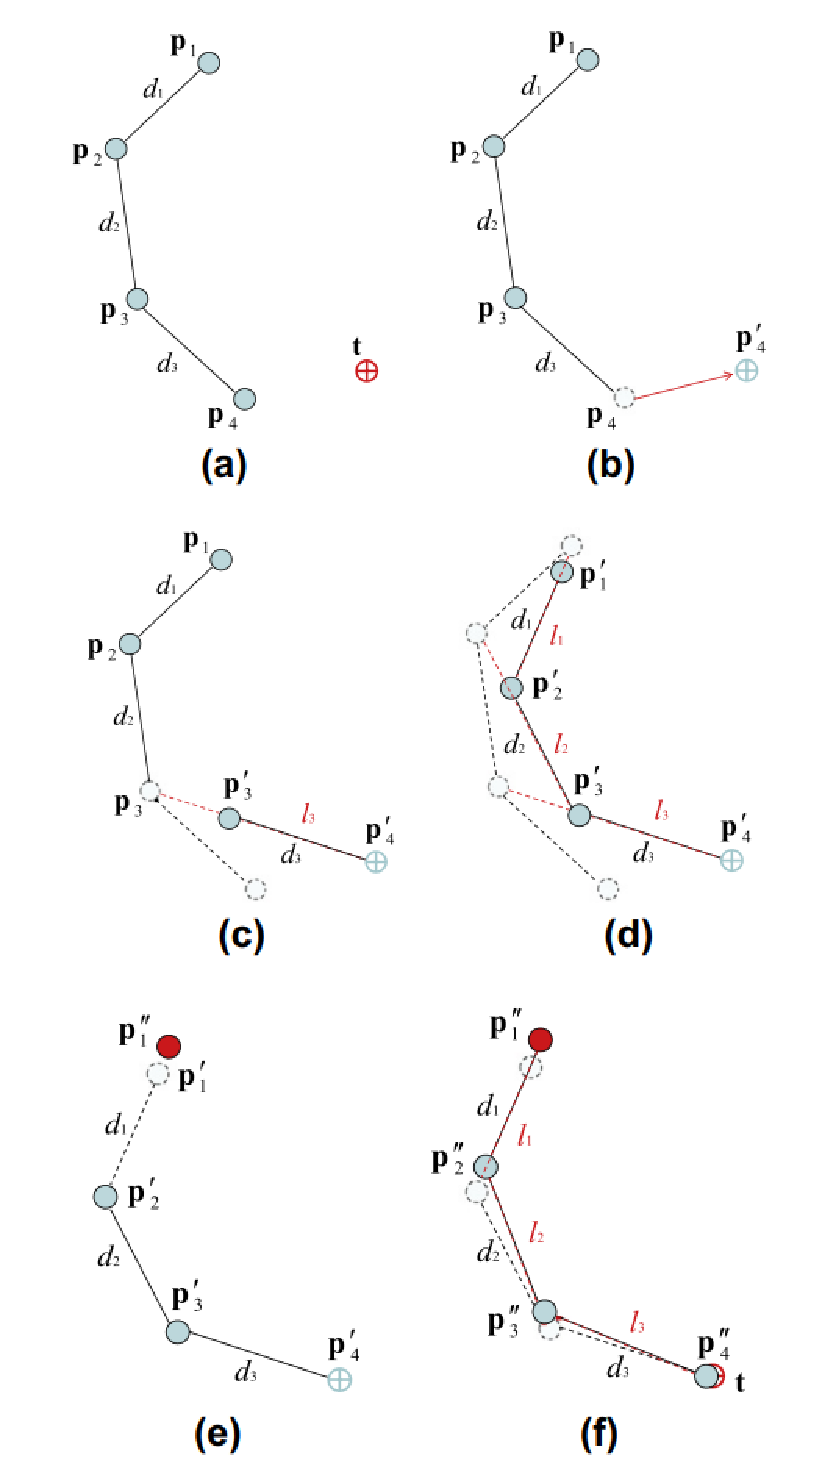
\includegraphics[width=2.5in]{images/FABRIK_Iteration.pdf}
\caption{
from \cite{aristidou_fabrik_2011}. An example of a full iteration of FABRIK for the case of a single target and 4 manipulator joints. (a) The initial position of the manipulator and the target, (b) move the end effector $\textbf{p}_4$ to the target, (c) find the joint $\textbf{p}'_3$ which lies on the line $l_3$ that passes through the points $\textbf{p}'_4$ and $\textbf{p}_3$, and has distance $d_3$ from the joint $\textbf{p}'_4$, (d) continue the algorithm for the rest of the joints, (e) the second stage of the algorithm: move the root joint $\textbf{p}'_1$ to its initial position, (f) repeat the same procedure but this time start from the base and move outwards to the end effector. The algorithm is repeated until the position of the end effector reaches the target or gets sufficiently close.
}
\label{fig:FABRIK_Iteration}
\end{figure}
\subsubsection{FABRIK}
Forward And Backward Reaching Inverse Kinematics (FABRIK)\cite{aristidou_fabrik_2011} is a heuristic method that iteratively adjusts the joint angles in both forward and backward directions until the end-effector reaches the desired position (Fig.\ref{fig:FABRIK_Iteration}) with an acceptable error margin.

\begin{figure}[!t]
\centering
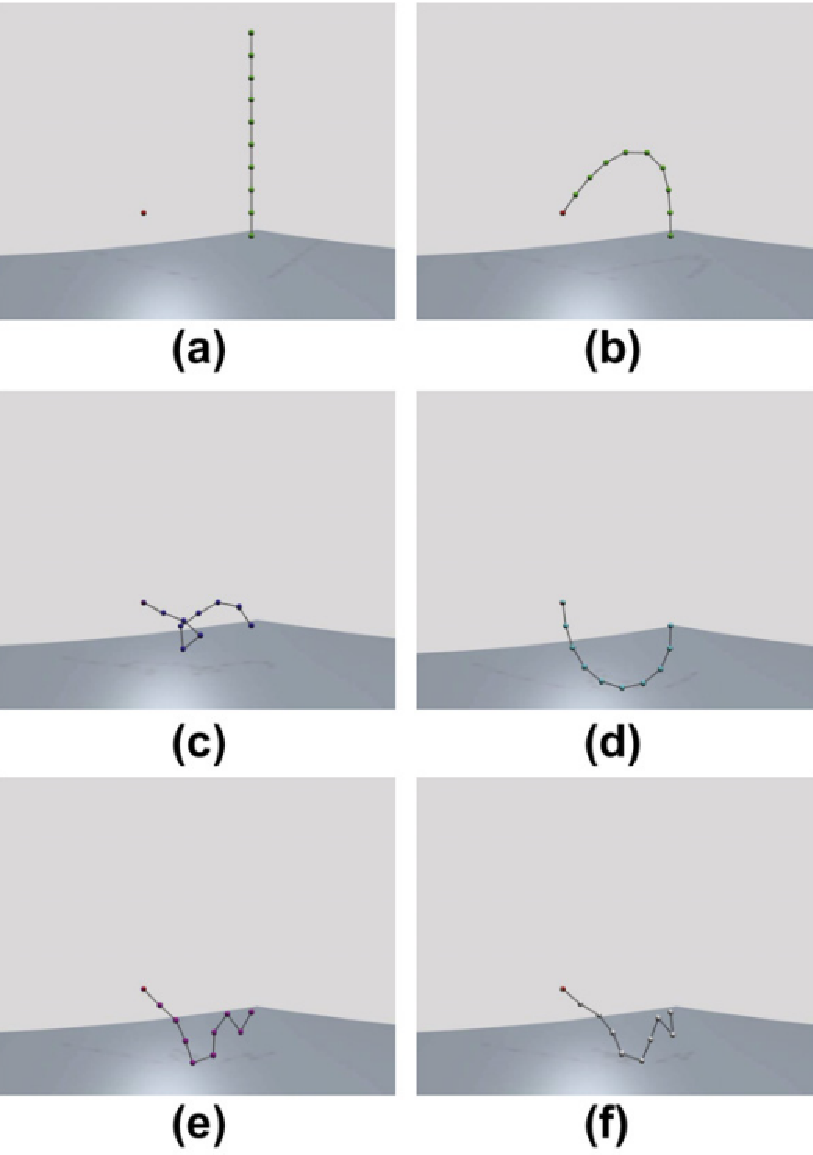
\includegraphics[width=2.5in]{images/FABRIK_Comparison.pdf}
\caption{
from \cite{aristidou_fabrik_2011}. Experimental solutions using some of the most popular IK methods. The kinematic chains consisted of 10 unconstrained joints, allowing 3 DOF on each joint. (a) Initial position, (b) FABRIK, (c) CCD, (d) Transpose, (e) DLS, (f) SDLS
}
\label{fig:FABRIK_Comparison}
\end{figure}

The bidirectional approach in FABRIK, and the iterative adjustments, make it suitable for solving multiple end-effector problems. Additionally, FABRIK reduces the potential for erratic motion (Fig. \ref{fig:FABRIK_Comparison}) compared to CCD by treating the kinematic chain as a whole in each iteration. FABRIK also exhibits linear time complexity in the number of iterations and the DOF. The FABRIK method is noted for its superior computational efficiency and speed\cite{aristidou_fabrik_2011} .

It is a popular choice for real-time applications in robotics, game development, and the animation industry\cite{aristidou_fabrik_2011}. The iterative nature of FABRIK allows it to adaptively adjust the joint angles based on the current state of the kinematic chain, thus generating more natural and smooth motions(Fig. \ref{fig:FABRIK_Comparison}). In spite of this, the quality of solutions still relies on the fine-tuning of parameters within the algorithm. Looking at an increasing pose precision of the end-effector in the dimension of $10^{-4}m$, FABRIK reveals an unstable convergence behavior\cite{xu_combined_2023}.

\subsubsection{Obstacle Avoidance with Heuristic methods}
Heuristic methods often incorporate strategies for avoiding obstacles while still reaching the target position. Like their Jacobian-based counterparts, heuristic methods have been extended for obstacle avoidance in inverse kinematics. This report will focus on the FABRIK method since it surpasses CCD in complexity, movement quality, and speed\cite{aristidou_fabrik_2011}. FABRIK also does not contain the constraints problem, is compatible with multiple end effectors, and is superior in all comparable aspects\cite{aristidou_fabrik_2011}. 
FABRIK has been modified to incorporate obstacle avoidance capabilities in \cite{tao_extending_2021}\cite{tao_collision-free_2017} and for continuum robots \cite{wu_novel_2022} and \cite{gerget_collision_2019} also introduced an extension. Still, we will concentrate on non-continuum robots in this report.

A two-step obstacle avoidance technique was proposed by \cite{tao_extending_2021} to extend the basic FABRIK method. Firstly, a heuristic approach is adopted to ensure the updated linkage bar, the root joint, and the target position in a line so that interference can be eliminated in most cases. Secondly, multiple random rotation strategies are applied to eliminate the interference that has not been eliminated in the first step.

However, the extended FABRIK method still needs to address the problem that the experimental results may vary for different tests due to adopting to avoid the obstacle. There are also some optimization approaches\cite{wu_crrik_2022}\cite{xie_obstacle_2020} that further improved FABRIK while maintaining the secondary task obstacle avoidance.

\subsubsection{Comparison of Heuristic and Jacobian methods}\label{Comparison of Heuristic and Jacobian methods}
Due to the IK's comparably low computation time a FABRIK surpasses all Jacobian methods by far in runtime \cite{xie_obstacle_2020}. Adding obstacle avoidance, we can also assume a faster calculation using the FABRIK method compared to the Jacobian method when looking at the given the time of 0.99s to 1.51s for a 5-link manipulator in \cite{kelemen_novel_2018} and ~0.07s to ~0.2s for a 4-link manipulator in\cite{tao_extending_2021}. In conclusion, using the FABRIK approach, we can assume more natural movements (Fig.\ref{fig:FABRIK_Comparison}) and faster calculation times. On top heuristic methods are free from singularities methods and therefore recommended when compared to any Jacobian method considering obstacle avoidance.


\subsection{Meta-Heuristic Methods}
We will define the class of Meta-Heuristic Methods for any Heuristic approach not explicitly designed for the IK problem. These methods have shown promising results, mainly due to their global search capability and the ability to handle multi-objective and multimodal optimization problems. Meta-heuristic methods offer a stochastic global optimization approach that will be discussed in the following section, often involving nature-inspired strategies. Their defining characteristic is their reliance on a general minimization function, which aids in their application across various complex and disparate problem domains. The function guides the search through the solution space to find an optimal or near-optimal solution, effectively minimizing the objective function, which in the case of inverse kinematics, would be to reduce the error between the desired and actual end-effector position. 
\begin{equation}
min\left( ||P_{cur} - P_{des}||^2 + ||R_{cur}-R_{des}||^2\right)
\end{equation}
where $P_{cur}$ is the current manipulator position, and $P_{des}$ is the target position of the end-effector. The subtraction is the Euclidean distance between $P_{cur}$ and $P_{des}$. Analogously, $R_{cur}$ is the current orientation of the manipulator, and $R_{des}$ is the target orientation. Optionally those terms can be weighted as used in \cite{tabandeh_adaptive_2010}.
Methods that will not be discussed include Simulated Annealing\cite{koker_neuro-simulated_2013}, Genetic Algorithm \cite{nearchou_solving_1998}, the Ant Colony Optimization\cite{chen_optimizing_2021}\cite{xu_trajectory_2023}, Bees Algorithm \cite{pham_learning_2008}\cite{dereli_simulation_2020}\cite{zhang_novel_2019}. and optimization methods mentioned in \ref{Jacobian Obstacle Avoidance}.

\subsubsection{Differential Evolution Algorithms}
Differential Evolution Algorithms(DEAs)\cite{storn_differential_1997} are a class of population-based stochastic algorithms for global optimization. The key idea behind DEAs is the generation of new candidate solutions by combining existing ones. Specifically, DEAs produce offspring by adding the weighted difference of two randomly selected solutions to a third one. The offspring are then evaluated and compete with the current generation's individuals for a place in the next generation:
\begin{enumerate}
  \item Initialization: A population of potential solutions is randomly initialized.
  \item Mutation: This stage generates a 'donor' vector by adding the weighted difference of two randomly chosen vectors to a third one.
  \item Crossover: This process combines the donor vector with a target vector to create a 'trial' vector.
  \item Selection: If the trial vector's fitness is greater than or equal to the target vector's fitness, the trial vector replaces the target vector in the next generation.
\end{enumerate}
A crucial aspect of DEAs is the control parameters: mutation scaling factor, crossover rate, and population size. The mutation scaling factor influences the rate at which the population evolves. The crossover rate affects the diversity of the offspring, while the population size determines the algorithm's ability to explore the solution space. Compared to Evolutionary Algorithms, DEAs specifically use vector difference operations and a simple arithmetic crossover to manipulate the population of solutions.
DEAs have proven effective in solving the IK problem \cite{zhang_research_2021}\cite{wu_huapeng_utilization_2000} due to their ability to handle non-linear, non-differentiable, multi-modal, and high-dimensional spaces. Despite their advantages, DEAs also have limitations, such as being sensitive to parameter settings and slow convergence in the later stages of optimization. That can be mitigated through adaptive or self-adaptive strategies dynamically adjusting the control parameters based on the algorithm's performance.

\subsubsection{Particle Swarm Optimization}
Particle Swarm Optimization (PSO)\cite{wang_particle_2018} is a meta-heuristic optimization technique that draws its inspiration from the social behavior of bird flocks or fish schools. PSO operates by maintaining a swarm of particles that traverse the search space. Each particle in the swarm represents a potential solution to the problem at hand. The position of a particle is updated based on its personal best solution and the global best solution found by the swarm so far. 
PSO is noted for its simplicity, ease of implementation, and the small number of parameters required. It has shown significant effectiveness in solving the IK problems \cite{yiyang_general_2021}\cite{Deng2021}. However, like most meta-heuristics, PSO can sometimes struggle with premature convergence and lack of diversity in the swarm. Various strategies, such as adaptive inertia weight, dynamic parameter adaptation, and hybridization with other algorithms, have been proposed to address these limitations\cite{yiyang_general_2021}.

\subsubsection{Obstacle Avoidance with Meta-Heuristic methods}
Similarly to the minimizing function for the Jacobian methods, the object function can easily be extended to avoid collision. The new formula can be expressed as follows:
\begin{equation}
min\left( ||P_{cur} - P_{des}||^2 + ||R_{cur}-R_{des}||^2 + \sum_{i=1}^m C_i\right)
\end{equation}
where $C_i$ is the penalty of the i-th collision and $m$ is the amount of collisions. When comparing the presented method, the initial ascertainment may be that their performance is similar. \cite{kacprzyk_particle_2008} showed that combining DEAs and PSO will further optimize runtime and accuracy. Due to the versatile nature of the algorithms, the combination of PSO and DEAs\cite{starke_efficient_2016} is also recommended for the IK problem considering obstacle avoidance

\subsubsection{Comparing Meta-Heuristic methods with Jacobian Methods and Heuristic methods}\label{Comparing All Section}
\begin{table}[ht]
\centering
\caption{Comparison of Jacobian, Heuristic, and Meta-Heuristic Methods}\label{Comparing all table}
\begin{tabular}{|c|c|c|c|}
\hline
\textbf{Method} & \textbf{Runtime} & \textbf{Singularity Robust} & \textbf{Scalability}\\
\hline
Jacobian & Medium & No & Low  \\
Heuristic & Low & Yes & Medium \\
Meta-Heuristic & High & Yes & High \\
\hline
\end{tabular}
\end{table}

As seen in Table \ref{Comparing all table} Meta-Heuristic methods do not have difficulties around singularities. However, based on the broad application possibilities, the runtime of the Meta-Heuristic methods is higher than the Jacobian methods. Being specifically designed for the IK problem, the Jacobian methods are more efficient. Thus, considering the scalability and implementation time, the Meta-Heuristic shine due to its adaptive nature. Further, it can be said that the Meta-Heuristic methods are more likely to avoid local minima due to their highly adapting nature and may therefore achieve a better target position while also coping with multiple end-effectors.

Comparing the Meta-Heuristic and Heuristic methods, we note that both methods are well-behaved around singularities. In contrast, the computational complexity is lower within the Heuristic methods since they were also designed for the IK Problem and prove a better efficiency. Even with this, the Meta-Heuristic methods may also result in a more precise target position when considering that Heuristic methods, especially with obstacle avoidance, may not find the optimal solution. In terms of scalability and ease of implementation, the Meta-Heuristic methods have the advantage compared to the Heuristic methods, which are not generally applicable.

In general, the Meta-Heuristic's robustness, easy implementation, and scalability make the Meta-Heuristic an excellent method candidate when the runtime is not important. Otherwise, the heuristic method can be recommended when prioritizing real-time usability.

\section{Conclusion and further restrictions}
In this report, we discussed the most common Jacobian, Heuristic, and Meta-Heuristic Methods and analyzed which may be the best option for different situations. Concluding the Meta-Heuristic method, e.g. a combination of PSO and DEAs, is recommended when the real-time calculation is not of the essence. If fast runtimes are essential, a Heuristic method, like an optimized form of FABRIK, is the best option. On top of that optimization techniques (\ref{Jacobian Obstacle Avoidance},\ref{Comparing All Section}) can be combined with those two methods, further reducing calculation time or the number of iterations.

When using those methods on robots in practice, additional factors must be considered. Some further restrictions concerning the inverse kinematic model's secondary task include optimizing execution time, Minimizing energy consumption, actuation limits, contact dynamics, obstacle detection, path planning, joint limits, or dynamics of a robot, and many more.

% use section* for acknowledgement
%\section*{Acknowledgment}
%The author would like to thank Jonathan Külz for his consultation and time as well as the TUM School of Computation, Information and Technology at Technical University Munich for the provided resources.

% trigger a \newpage just before the given reference
% number - used to balance the columns on the last page
% adjust value as needed - may need to be readjusted if
% the document is modified later
%\IEEEtriggeratref{8}
% The "triggered" command can be changed if desired:
%\IEEEtriggercmd{\enlargethispage{-5in}}



% references section

% can use a bibliography generated by BibTeX as a .bbl file
% BibTeX documentation can be easily obtained at:
% http://www.ctan.org/tex-archive/biblio/bibtex/contrib/doc/
% The IEEEtran BibTeX style support page is at:
% http://www.michaelshell.org/tex/ieeetran/bibtex/
%\bibliographystyle{IEEEtran}
\bibliographystyle{IEEEtran}
% argument is your BibTeX string definitions and bibliography database(s)
\bibliography{Bibliography/Report}

\end{document}
